\section{Registers}

Since the registers are one of the most important entities in MMIX, they are explained at first. MMIX has special, global and local registers, which will be described one after another in this section.

\subsection{Special Registers}

MMIX provides 32 special registers in an array called $sp$ in this thesis\footnote{The special registers may be put in the first 32 slots of the global register array, which is the reason why \sr{G} is always at least 32, as it will be mentioned in the next section. But actually, this is not enforced.}. Most of them will be introduced later as soon as the associated concept or instruction is described. The other ones, that do not fit into a certain category or are very important, are explained here.

\begin{itemize}
	\item \sr{A} - Arithmetic status register:\\
	Since \sr{A} affects many instructions, it is explained first. Its layout is:
	
	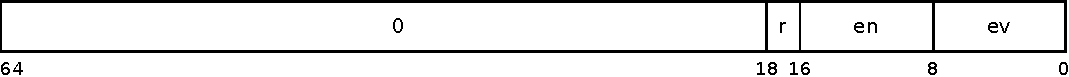
\includegraphics[width=\linewidth]{img/rA-crop.pdf}
	
	The fields $en$ and $ev$ contain \i{enable} and \i{event} bits, both called abbreviated "DVWIOUZX from left to right, where D stands for integer divide check, V for integer overflow, W for float-to-fix overflow, I for invalid operation, O for floating overflow, U for floating underflow, Z for floating division by zero, and X for floating inexact." \citep[pg. 26]{mmix-doc}
	The enable bits control whether an \glslink{Exception}{AE} is raised as soon as the corresponding exceptional condition occurs, while the event bits will be set if no \glslink{Exception}{AE} is raised.
	The field $r$ specifies the rounding mode that is used for floating point numbers, where $00_2$ means round near, $01_2$ round toward zero, $10_2$ round toward $+\infty$ and $11_2$ round toward $-\infty$. All other bits are defined to be zero. \citep[pg. 15 and 26]{mmix-doc}
	
	\item \sr{C} - Cycle counter:\\
	As the name suggests, MMIX increases this special register on every cycle by 1. It can be used to measure the performance of a code snippet, for example. \citep[pg. 32]{mmix-doc}
	\item \sr{I} - Interval counter:\\
	The special register \sr{I} is decreased by 1 on every cycle and causes an \i{interval \glslink{Interrupt}{interrupt}} as soon as it reaches zero. It can also be used for runtime analysis. \citep[pg. 32]{mmix-doc}
	\item \sr{U} - Usage counter:\\
	Register \sr{U} is structured in the following way:
	
	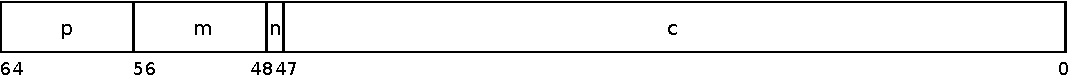
\includegraphics[width=\linewidth]{img/rU-crop.pdf}
	
	The usage count $c$ is increased whenever $op~\&~m = p$, where $op$ is the opcode of an instruction. The bit $n$ indicates whether it should also be done when the \glslink{PC}{instruction pointer} is in the privileged space. \citep[pg. 32]{mmix-doc}
	\item \sr{F} - Failure location register:\\
	This register holds the physical memory address when a parity error or other kinds of memory faults occur. Since an MMIX implementation may use caching, the instruction that caused this error might be long gone before it is detected. \citep[pg. 40]{mmix-doc}
	\item \sr{N} - Serial number:\\
	Register \sr{N} identifies the particular MMIX implementation and is structured as follows:
	
	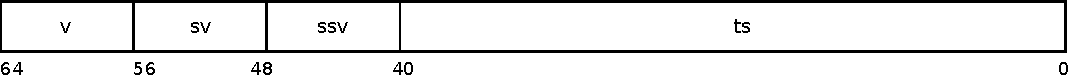
\includegraphics[width=\linewidth]{img/rN-crop.pdf}
	
	The fields $v$, $sv$ and $ssv$ specify the MMIX architecture version. This thesis describes version 1, subversion 0 and subsubversion 0, \ie 1.0.0. The field $ts$ holds the number of seconds from 01/01/1970, 00:00:00 GMT to the date the particular instance of MMIX was built on. \citep[pg. 32]{mmix-doc}
\end{itemize}

\noindent MMIX provides two instructions to read from or write to a special register.

\instrtbl
	{\mi{GET \$X,Z}}
	{\dr{X} $\leftarrow$ \spr{Z}}
\noindent The instruction \mi{GET} sets \dr{X} to the value of special register `Z`. MMIX does not keep secrets from the user, \ie all special registers are readable -- even in user mode. \citep[pg. 34]{mmix-doc}

\instrtbl
	{\mi{PUT X,\$Z|Z}}
	{\spr{X} $\leftarrow$ \udrim{Z}}
\noindent \mi{PUT} sets special register `X` to either \dr{Z} or the \glslink{Immediate Value}{immediate value} `Z`. The registers \sr{C}, \sr{N}, \sr{O} and \sr{S} are not writeable in general. \sr{I}, \sr{T}, \sr{TT}, \sr{K}, \sr{Q}, \sr{U} and \sr{V} are writeable in privileged mode only. Additionally, in \sr{A} all bits except \haddrt{3}{FFFF} have to be zero, \sr{G} can't be less than $max(\sr{L},32)$ and not greater than 255. Furthermore, \sr{L} can't be increased with \mi{PUT} and bits in the \i{\glslink{Interrupt}{interrupt} request register} \sr{Q}, that have been set by MMIX since the last execution of \mi{GET \dr{X},\sr{Q}}, can not be unset. In this way, no \glslink{Exception}{PE}, \glslink{Exception}{ME} or \glslink{Interrupt}{interrupt} bit can be lost by accident.\footnote{The restrictions will become more clear as soon as the concepts and instructions working with these registers have been explained.} \citep[pg. 34]{mmix-doc}

\subsection{Global and Local Registers}

MMIX maintains two banks of registers. One for global registers, called $g$, which has at most 256 slots. The other one for local registers, called $l$, which has $2^n$ slots, where $n$ is between 8 and 10. Both can be accessed by the so called \i{dynamic registers} \dr{0}, \dr{1}, \dots, \dr{255}. MMIX uses the special register \sr{G} to separate them. \sr{G} is always at least 32 at at most 255. When saying \dr{X}, it denotes a global register whenever `X` is greater or equal to \sr{G}. It will denote a local register if it is less than \sr{G}. \citep[pg. 22]{mmix-doc}

Additionally, \sr{L} splits the local registers in two categories. The registers \dr{0}, \dots, \dr{(rL - 1)} are the local registers that are currently in use. The other ones, \dr{(rL)}, \dots, \dr{(rG - 1)}, are called \i{marginal}. If such a register is read, it will always yield zero. If \dr{X} is written, whereas $\sr{L} \le {\tt X} < \sr{G}$, the registers \dr{(rL)}, \dots, \dr{(X - 1)} will be set to zero, \dr{X} will be set to the desired value and \sr{L} will be set to ${\tt X} + 1$. \citep[pg. 22]{mmix-doc}

For example, if \sr{L} is 4 and \sr{G} is 64,
\begin{itemize}
	\item reading \dr{3} will yield the value of $l[3]$,
	\item reading \dr{4} will yield 0,
	\item writing 12 to \dr{5} will set $l[4]$ to 0, $l[5]$ to 12 and \sr{L} to 6,
	\item reading \dr{64} will yield the value of $g[64]$ and
	\item writing 100 to \dr{70} will set $g[70]$ to 100.
\end{itemize}

